\hypertarget{implementation-of-scheffe-wald-test-on-a-penalty-analysis}{%
\section{Implementation of Scheffe-Wald test on a Penalty
analysis}\label{implementation-of-scheffe-wald-test-on-a-penalty-analysis}}

\begin{lstlisting}[language=Python]
import pandas as pd
import numpy as np
import os
import sys
from pathlib import Path

import pandas as pd
import numpy as np
from typing import Dict, List, Tuple
import matplotlib.pyplot as plt
import seaborn as sns
\end{lstlisting}

\begin{lstlisting}[language=Python]
CURRENT_PATH = Path.cwd()
MAIN_DIR = os.path.abspath(CURRENT_PATH.parent)
INPUT_DIR = os.path.join(CURRENT_PATH, 'data')
\end{lstlisting}

\begin{lstlisting}[language=Python]
sys.path.append(MAIN_DIR)

from MultipleTesting.multiple_comparisons import *
from MultipleTesting.visualization import *
\end{lstlisting}

\hypertarget{read-data}{%
\section{READ DATA}\label{read-data}}

\begin{lstlisting}[language=Python]
df = pd.read_csv(os.path.join(INPUT_DIR,'dt_compMult_formula_182.csv' ))

CONTEOS = (
    df
    .groupby(['atributo','nivel'])['sbj_num']
    .nunique()
    .reset_index()
)
\end{lstlisting}

\begin{lstlisting}[language=Python]
OVERALL_LIKING = pd.read_csv(os.path.join(INPUT_DIR, 'dt_penalty.csv'))
OVERALL_LIKING['atributo'] = OVERALL_LIKING['atributo'].str.lower()
OVERALL_LIKING['nivel'] = OVERALL_LIKING['nivel'].str.upper()
\end{lstlisting}

\begin{lstlisting}[language=Python]
def get_counts_for_attribute(df_counts: pd.DataFrame, measurement: str, atributo: str) -> list:
    """
    Extracts counts in order JAR, TL, TM for a given attribute.
    """
    counts = df_counts[df_counts['atributo'] == atributo].sort_values('nivel')
    return [
        counts[counts['nivel'] == 'JAR'][measurement].iloc[0],
        counts[counts['nivel'] == 'TL'][measurement].iloc[0],
        counts[counts['nivel'] == 'TM'][measurement].iloc[0]
    ]
\end{lstlisting}

\begin{lstlisting}[language=Python]
def plot_penalty_heatmap(df_ol: pd.DataFrame, df_counts: pd.DataFrame, title: str = "Penalty Analysis Heatmap"):
    """
    Creates a heatmap visualization using DataFrames.
    """
    # Prepare data for proportions
    prop_data = df_counts.pivot_table(
        values='sbj_num', 
        index='atributo', 
        columns='nivel', 
        aggfunc='sum'
    )
    
    # Calculate proportions
    total_responses = prop_data.sum(axis=1)
    prop_data = prop_data.div(total_responses, axis=0)
    
    # Calculate overall liking differences
    ol_data = df_ol.pivot_table(
        values='overall_liking',
        index='atributo',
        columns='nivel'
    )
    
    ol_diffs = pd.DataFrame({
        'TL_diff': ol_data['JAR'] - ol_data['TL'],
        'TM_diff': ol_data['JAR'] - ol_data['TM']
    })
    
    # Create figure with two subplots
    fig, (ax1, ax2) = plt.subplots(1, 2, figsize=(15, 8), gridspec_kw={'width_ratios': [1.5, 1]})
    
    # Plot proportions heatmap
    sns.heatmap(prop_data, 
                annot=True, 
                fmt='.3f',
                cmap='YlOrRd',
                ax=ax1)
    ax1.set_title('Proporción de Respuestas', pad=20)
    
    # Plot overall liking differences heatmap
    sns.heatmap(ol_diffs,
                annot=True,
                fmt='.2f',
                cmap='RdYlBu_r',
                center=0,
                ax=ax2)
    ax2.set_title('Diferencias Overall Liking\n(vs JAR)', pad=20)
    
    plt.suptitle(title, fontsize=14, y=1.05)
    plt.tight_layout()
    return fig, (ax1, ax2)

plot_penalty_heatmap(OVERALL_LIKING, CONTEOS, title="")
\end{lstlisting}

\begin{lstlisting}
(<Figure size 1500x800 with 4 Axes>,
 (<Axes: title={'center': 'Proporción de Respuestas'}, xlabel='nivel', ylabel='atributo'>,
  <Axes: title={'center': 'Diferencias Overall Liking\n(vs JAR)'}, ylabel='atributo'>))
\end{lstlisting}

\begin{figure}
\centering
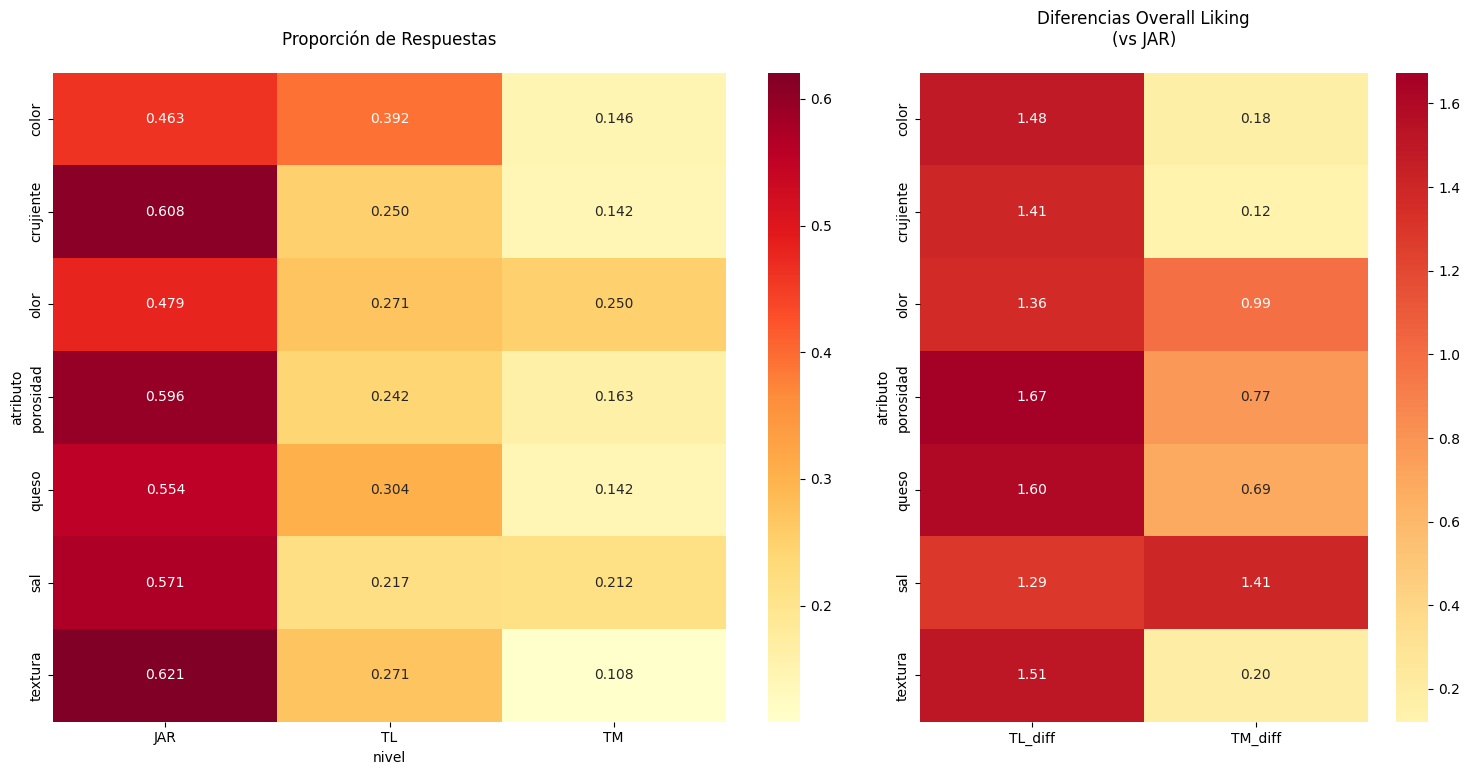
\includegraphics{implementation_files/implementation_8_1.png}
\caption{png}
\end{figure}

\begin{lstlisting}[language=Python]
df_result = pd.DataFrame()
alpha = 0.1

# Matriz de contraste para las comparaciones
A = np.array([
    [1, -1, 0],   # JAR vs TL
    [1, 0, -1],   # JAR vs TM
])

for attribute in CONTEOS['atributo'].unique():
    counts = get_counts_for_attribute(CONTEOS, 'sbj_num', attribute) # porportions are computed inside

    test = StatisticalTest(counts, alpha=alpha)

    bonf_results = test.bonferroni_confidence_intervals()
    tukey_results = test.tukey_confidence_intervals()
    scheffe_results = test.scheffe_wald_test(A)

    all_results = [scheffe_results, bonf_results, tukey_results]

    # Print results 
    print(str.upper(attribute),"*" * 70)
    print_test_results(all_results)
    print("=" * 80)

    for method in all_results:
        result = format_test_results_df(method)
        result['attribute'] = attribute
        
        df_result = pd.concat([df_result, result]) 

df_result['p_i-p_j'] = df_result['p_i-p_j'].str.replace('0','JAR').str.replace('1','TL').str.replace('2','TM').str.replace('p_','')
\end{lstlisting}

\begin{lstlisting}
COLOR **********************************************************************

--------------------------------------------------------------------------------
Scheffé-Wald Results:
--------------------------------------------------------------------------------
Overall p-value: 0.0000
Test statistic: 68.5999
Degrees of freedom: (df=2)

Pairwise Comparisons (90.0% Confidence Intervals):
Category i Category j  Difference   CI Lower   CI Upper   p-value  
--------------------------------------------------------------------------------
    0          1         0.0708     -0.0748     0.2164     0.2337  
    0          2         0.3167      0.2040     0.4293     0.0000  
--------------------------------------------------------------------------------


--------------------------------------------------------------------------------
Bonferroni Results:
--------------------------------------------------------------------------------
Overall p-value: 0.0000
Test statistic: 8.0308
Degrees of freedom: (num=1, error=239.0)

Pairwise Comparisons (90.0% Confidence Intervals):
Category i Category j  Difference   CI Lower   CI Upper   p-value  
--------------------------------------------------------------------------------
    0          1         0.0708     -0.0250     0.1667     0.3474  
    0          2         0.3167      0.2328     0.4006     0.0000  
    1          2         0.2458      0.1631     0.3286     0.0000  
--------------------------------------------------------------------------------


--------------------------------------------------------------------------------
Tukey Results:
--------------------------------------------------------------------------------
Overall p-value: 0.0000
Test statistic: 11.3573
Degrees of freedom: (num=2, error=237.0)

Pairwise Comparisons (90.0% Confidence Intervals):
Category i Category j  Difference   CI Lower   CI Upper   p-value  
--------------------------------------------------------------------------------
    0          1         0.0708     -0.0221     0.1637     0.2595  
    0          2         0.3167      0.2353     0.3980     0.0000  
    1          2         0.2458      0.1656     0.3260     0.0000  
--------------------------------------------------------------------------------

================================================================================
CRUJIENTE **********************************************************************

--------------------------------------------------------------------------------
Scheffé-Wald Results:
--------------------------------------------------------------------------------
Overall p-value: 0.0000
Test statistic: 98.7376
Degrees of freedom: (df=2)

Pairwise Comparisons (90.0% Confidence Intervals):
Category i Category j  Difference   CI Lower   CI Upper   p-value  
--------------------------------------------------------------------------------
    0          1         0.3583      0.2233     0.4933     0.0000  
    0          2         0.4667      0.3514     0.5819     0.0000  
--------------------------------------------------------------------------------


--------------------------------------------------------------------------------
Bonferroni Results:
--------------------------------------------------------------------------------
Overall p-value: 0.0000
Test statistic: 12.0516
Degrees of freedom: (num=1, error=239.0)

Pairwise Comparisons (90.0% Confidence Intervals):
Category i Category j  Difference   CI Lower   CI Upper   p-value  
--------------------------------------------------------------------------------
    0          1         0.3583      0.2687     0.4480     0.0000  
    0          2         0.4667      0.3843     0.5491     0.0000  
    1          2         0.1083      0.0320     0.1847     0.0076  
--------------------------------------------------------------------------------


--------------------------------------------------------------------------------
Tukey Results:
--------------------------------------------------------------------------------
Overall p-value: 0.0000
Test statistic: 17.0435
Degrees of freedom: (num=2, error=237.0)

Pairwise Comparisons (90.0% Confidence Intervals):
Category i Category j  Difference   CI Lower   CI Upper   p-value  
--------------------------------------------------------------------------------
    0          1         0.3583      0.2715     0.4452     0.0000  
    0          2         0.4667      0.3868     0.5465     0.0000  
    1          2         0.1083      0.0343     0.1823     0.0079  
--------------------------------------------------------------------------------

================================================================================
OLOR **********************************************************************

--------------------------------------------------------------------------------
Scheffé-Wald Results:
--------------------------------------------------------------------------------
Overall p-value: 0.0000
Test statistic: 20.7804
Degrees of freedom: (df=2)

Pairwise Comparisons (90.0% Confidence Intervals):
Category i Category j  Difference   CI Lower   CI Upper   p-value  
--------------------------------------------------------------------------------
    0          1         0.2083      0.0755     0.3411     0.0001  
    0          2         0.2292      0.0992     0.3591     0.0000  
--------------------------------------------------------------------------------


--------------------------------------------------------------------------------
Bonferroni Results:
--------------------------------------------------------------------------------
Overall p-value: 0.0000
Test statistic: 5.3701
Degrees of freedom: (num=1, error=239.0)

Pairwise Comparisons (90.0% Confidence Intervals):
Category i Category j  Difference   CI Lower   CI Upper   p-value  
--------------------------------------------------------------------------------
    0          1         0.2083      0.1165     0.3002     0.0000  
    0          2         0.2292      0.1384     0.3200     0.0000  
    1          2         0.0208     -0.0644     0.1061     1.0000  
--------------------------------------------------------------------------------


--------------------------------------------------------------------------------
Tukey Results:
--------------------------------------------------------------------------------
Overall p-value: 0.0000
Test statistic: 7.5945
Degrees of freedom: (num=2, error=237.0)

Pairwise Comparisons (90.0% Confidence Intervals):
Category i Category j  Difference   CI Lower   CI Upper   p-value  
--------------------------------------------------------------------------------
    0          1         0.2083      0.1193     0.2973     0.0000  
    0          2         0.2292      0.1412     0.3172     0.0000  
    1          2         0.0208     -0.0618     0.1034     0.8616  
--------------------------------------------------------------------------------

================================================================================
POROSIDAD **********************************************************************

--------------------------------------------------------------------------------
Scheffé-Wald Results:
--------------------------------------------------------------------------------
Overall p-value: 0.0000
Test statistic: 79.2026
Degrees of freedom: (df=2)

Pairwise Comparisons (90.0% Confidence Intervals):
Category i Category j  Difference   CI Lower   CI Upper   p-value  
--------------------------------------------------------------------------------
    0          1         0.3542      0.2208     0.4875     0.0000  
    0          2         0.4333      0.3140     0.5527     0.0000  
--------------------------------------------------------------------------------


--------------------------------------------------------------------------------
Bonferroni Results:
--------------------------------------------------------------------------------
Overall p-value: 0.0000
Test statistic: 10.9348
Degrees of freedom: (num=1, error=239.0)

Pairwise Comparisons (90.0% Confidence Intervals):
Category i Category j  Difference   CI Lower   CI Upper   p-value  
--------------------------------------------------------------------------------
    0          1         0.3542      0.2647     0.4436     0.0000  
    0          2         0.4333      0.3490     0.5177     0.0000  
    1          2         0.0792      0.0015     0.1568     0.0900  
--------------------------------------------------------------------------------


--------------------------------------------------------------------------------
Tukey Results:
--------------------------------------------------------------------------------
Overall p-value: 0.0000
Test statistic: 15.4641
Degrees of freedom: (num=2, error=237.0)

Pairwise Comparisons (90.0% Confidence Intervals):
Category i Category j  Difference   CI Lower   CI Upper   p-value  
--------------------------------------------------------------------------------
    0          1         0.3542      0.2675     0.4409     0.0000  
    0          2         0.4333      0.3516     0.5151     0.0000  
    1          2         0.0792      0.0039     0.1544     0.0785  
--------------------------------------------------------------------------------

================================================================================
QUESO **********************************************************************

--------------------------------------------------------------------------------
Scheffé-Wald Results:
--------------------------------------------------------------------------------
Overall p-value: 0.0000
Test statistic: 84.0268
Degrees of freedom: (df=2)

Pairwise Comparisons (90.0% Confidence Intervals):
Category i Category j  Difference   CI Lower   CI Upper   p-value  
--------------------------------------------------------------------------------
    0          1         0.2500      0.1090     0.3910     0.0000  
    0          2         0.4125      0.2979     0.5271     0.0000  
--------------------------------------------------------------------------------


--------------------------------------------------------------------------------
Bonferroni Results:
--------------------------------------------------------------------------------
Overall p-value: 0.0000
Test statistic: 10.5248
Degrees of freedom: (num=1, error=239.0)

Pairwise Comparisons (90.0% Confidence Intervals):
Category i Category j  Difference   CI Lower   CI Upper   p-value  
--------------------------------------------------------------------------------
    0          1         0.2500      0.1570     0.3430     0.0000  
    0          2         0.4125      0.3291     0.4959     0.0000  
    1          2         0.1625      0.0832     0.2418     0.0000  
--------------------------------------------------------------------------------


--------------------------------------------------------------------------------
Tukey Results:
--------------------------------------------------------------------------------
Overall p-value: 0.0000
Test statistic: 14.8843
Degrees of freedom: (num=2, error=237.0)

Pairwise Comparisons (90.0% Confidence Intervals):
Category i Category j  Difference   CI Lower   CI Upper   p-value  
--------------------------------------------------------------------------------
    0          1         0.2500      0.1598     0.3402     0.0000  
    0          2         0.4125      0.3317     0.4933     0.0000  
    1          2         0.1625      0.0857     0.2393     0.0001  
--------------------------------------------------------------------------------

================================================================================
SAL **********************************************************************

--------------------------------------------------------------------------------
Scheffé-Wald Results:
--------------------------------------------------------------------------------
Overall p-value: 0.0000
Test statistic: 55.2824
Degrees of freedom: (df=2)

Pairwise Comparisons (90.0% Confidence Intervals):
Category i Category j  Difference   CI Lower   CI Upper   p-value  
--------------------------------------------------------------------------------
    0          1         0.3542      0.2256     0.4827     0.0000  
    0          2         0.3583      0.2305     0.4862     0.0000  
--------------------------------------------------------------------------------


--------------------------------------------------------------------------------
Bonferroni Results:
--------------------------------------------------------------------------------
Overall p-value: 0.0000
Test statistic: 8.6451
Degrees of freedom: (num=1, error=239.0)

Pairwise Comparisons (90.0% Confidence Intervals):
Category i Category j  Difference   CI Lower   CI Upper   p-value  
--------------------------------------------------------------------------------
    0          1         0.3542      0.2657     0.4426     0.0000  
    0          2         0.3583      0.2701     0.4465     0.0000  
    1          2         0.0042     -0.0756     0.0839     1.0000  
--------------------------------------------------------------------------------


--------------------------------------------------------------------------------
Tukey Results:
--------------------------------------------------------------------------------
Overall p-value: 0.0000
Test statistic: 12.2261
Degrees of freedom: (num=2, error=237.0)

Pairwise Comparisons (90.0% Confidence Intervals):
Category i Category j  Difference   CI Lower   CI Upper   p-value  
--------------------------------------------------------------------------------
    0          1         0.3542      0.2684     0.4399     0.0000  
    0          2         0.3583      0.2729     0.4438     0.0000  
    1          2         0.0042     -0.0731     0.0815     0.9932  
--------------------------------------------------------------------------------

================================================================================
TEXTURA **********************************************************************

--------------------------------------------------------------------------------
Scheffé-Wald Results:
--------------------------------------------------------------------------------
Overall p-value: 0.0000
Test statistic: 147.5684
Degrees of freedom: (df=2)

Pairwise Comparisons (90.0% Confidence Intervals):
Category i Category j  Difference   CI Lower   CI Upper   p-value  
--------------------------------------------------------------------------------
    0          1         0.3500      0.2114     0.4886     0.0000  
    0          2         0.5125      0.4046     0.6204     0.0000  
--------------------------------------------------------------------------------


--------------------------------------------------------------------------------
Bonferroni Results:
--------------------------------------------------------------------------------
Overall p-value: 0.0000
Test statistic: 13.7795
Degrees of freedom: (num=1, error=239.0)

Pairwise Comparisons (90.0% Confidence Intervals):
Category i Category j  Difference   CI Lower   CI Upper   p-value  
--------------------------------------------------------------------------------
    0          1         0.3500      0.2596     0.4404     0.0000  
    0          2         0.5125      0.4334     0.5916     0.0000  
    1          2         0.1625      0.0880     0.2370     0.0000  
--------------------------------------------------------------------------------


--------------------------------------------------------------------------------
Tukey Results:
--------------------------------------------------------------------------------
Overall p-value: 0.0000
Test statistic: 19.4871
Degrees of freedom: (num=2, error=237.0)

Pairwise Comparisons (90.0% Confidence Intervals):
Category i Category j  Difference   CI Lower   CI Upper   p-value  
--------------------------------------------------------------------------------
    0          1         0.3500      0.2624     0.4376     0.0000  
    0          2         0.5125      0.4358     0.5892     0.0000  
    1          2         0.1625      0.0903     0.2347     0.0000  
--------------------------------------------------------------------------------

================================================================================
\end{lstlisting}

\begin{lstlisting}[language=Python]
df_result.to_csv(os.path.join(MAIN_DIR, 'test_results.csv'))
\end{lstlisting}

\begin{lstlisting}[language=Python]
colors = {'Scheffé-Wald': '#FF6B6B', 'Bonferroni': '#4ECDC4', 'Tukey': '#45B7D1'}
markers = {'Scheffé-Wald': 'o', 'Bonferroni': 's', 'Tukey': 'D'}
\end{lstlisting}

\begin{lstlisting}[language=Python]

fig = plt.figure(figsize=(15, 10))
attributes = df_result['attribute'].unique()
n_attrs = len(attributes)
rows = int(np.ceil(n_attrs/2))
fig, axes = plt.subplots(rows, 2, figsize=(15, 5*rows))
axes = axes.flatten()

# Plot for each attribute
for idx, attr in enumerate(attributes):
    ax = axes[idx]
    attr_data = df_result[(df_result['attribute'] == attr ) & (df_result['p_i-p_j'] != 'TL-TM')]
    
    y_positions = []
    y_labels = []
    current_pos = 0
    
    for comp in attr_data['p_i-p_j'].unique():
        comp_data = attr_data[attr_data['p_i-p_j'] == comp]
        
        # Add small offset for each test method
        for i, (_, row) in enumerate(comp_data.iterrows()):
            offset = i * 0.3 - (len(comp_data) - 1) * 0.15  # Center the methods
            y_pos = current_pos + offset
            
            ax.errorbar(
                x=row['diff'],
                y=y_pos,
                xerr=[[row['diff'] - row['conf_low']], [row['conf_hi'] - row['diff']]],
                fmt=markers[row['test']],
                color=colors[row['test']],
                capsize=5,
                label=row['test'] if current_pos == 0 else "",
                markersize=8
            )
            
        y_positions.append(current_pos)
        y_labels.append(comp)
        current_pos += 2.0  # Space between comparisons
    
    ax.axvline(x=0, color='gray', linestyle='--', alpha=0.5)
    ax.set_yticks(y_positions)
    ax.set_yticklabels(y_labels)
    ax.set_xlabel('Difference in Proportions')
    ax.set_title(f'Attribute: {attr}')
    ax.grid(True, alpha=0.3)
    
    if idx == 0:
        ax.legend()

# Remove empty subplots
for idx in range(len(attributes), len(axes)):
    fig.delaxes(axes[idx])

plt.tight_layout(h_pad=2.0, w_pad=2.0)
plt.show()
\end{lstlisting}

\begin{lstlisting}
<Figure size 1500x1000 with 0 Axes>
\end{lstlisting}

\begin{figure}
\centering
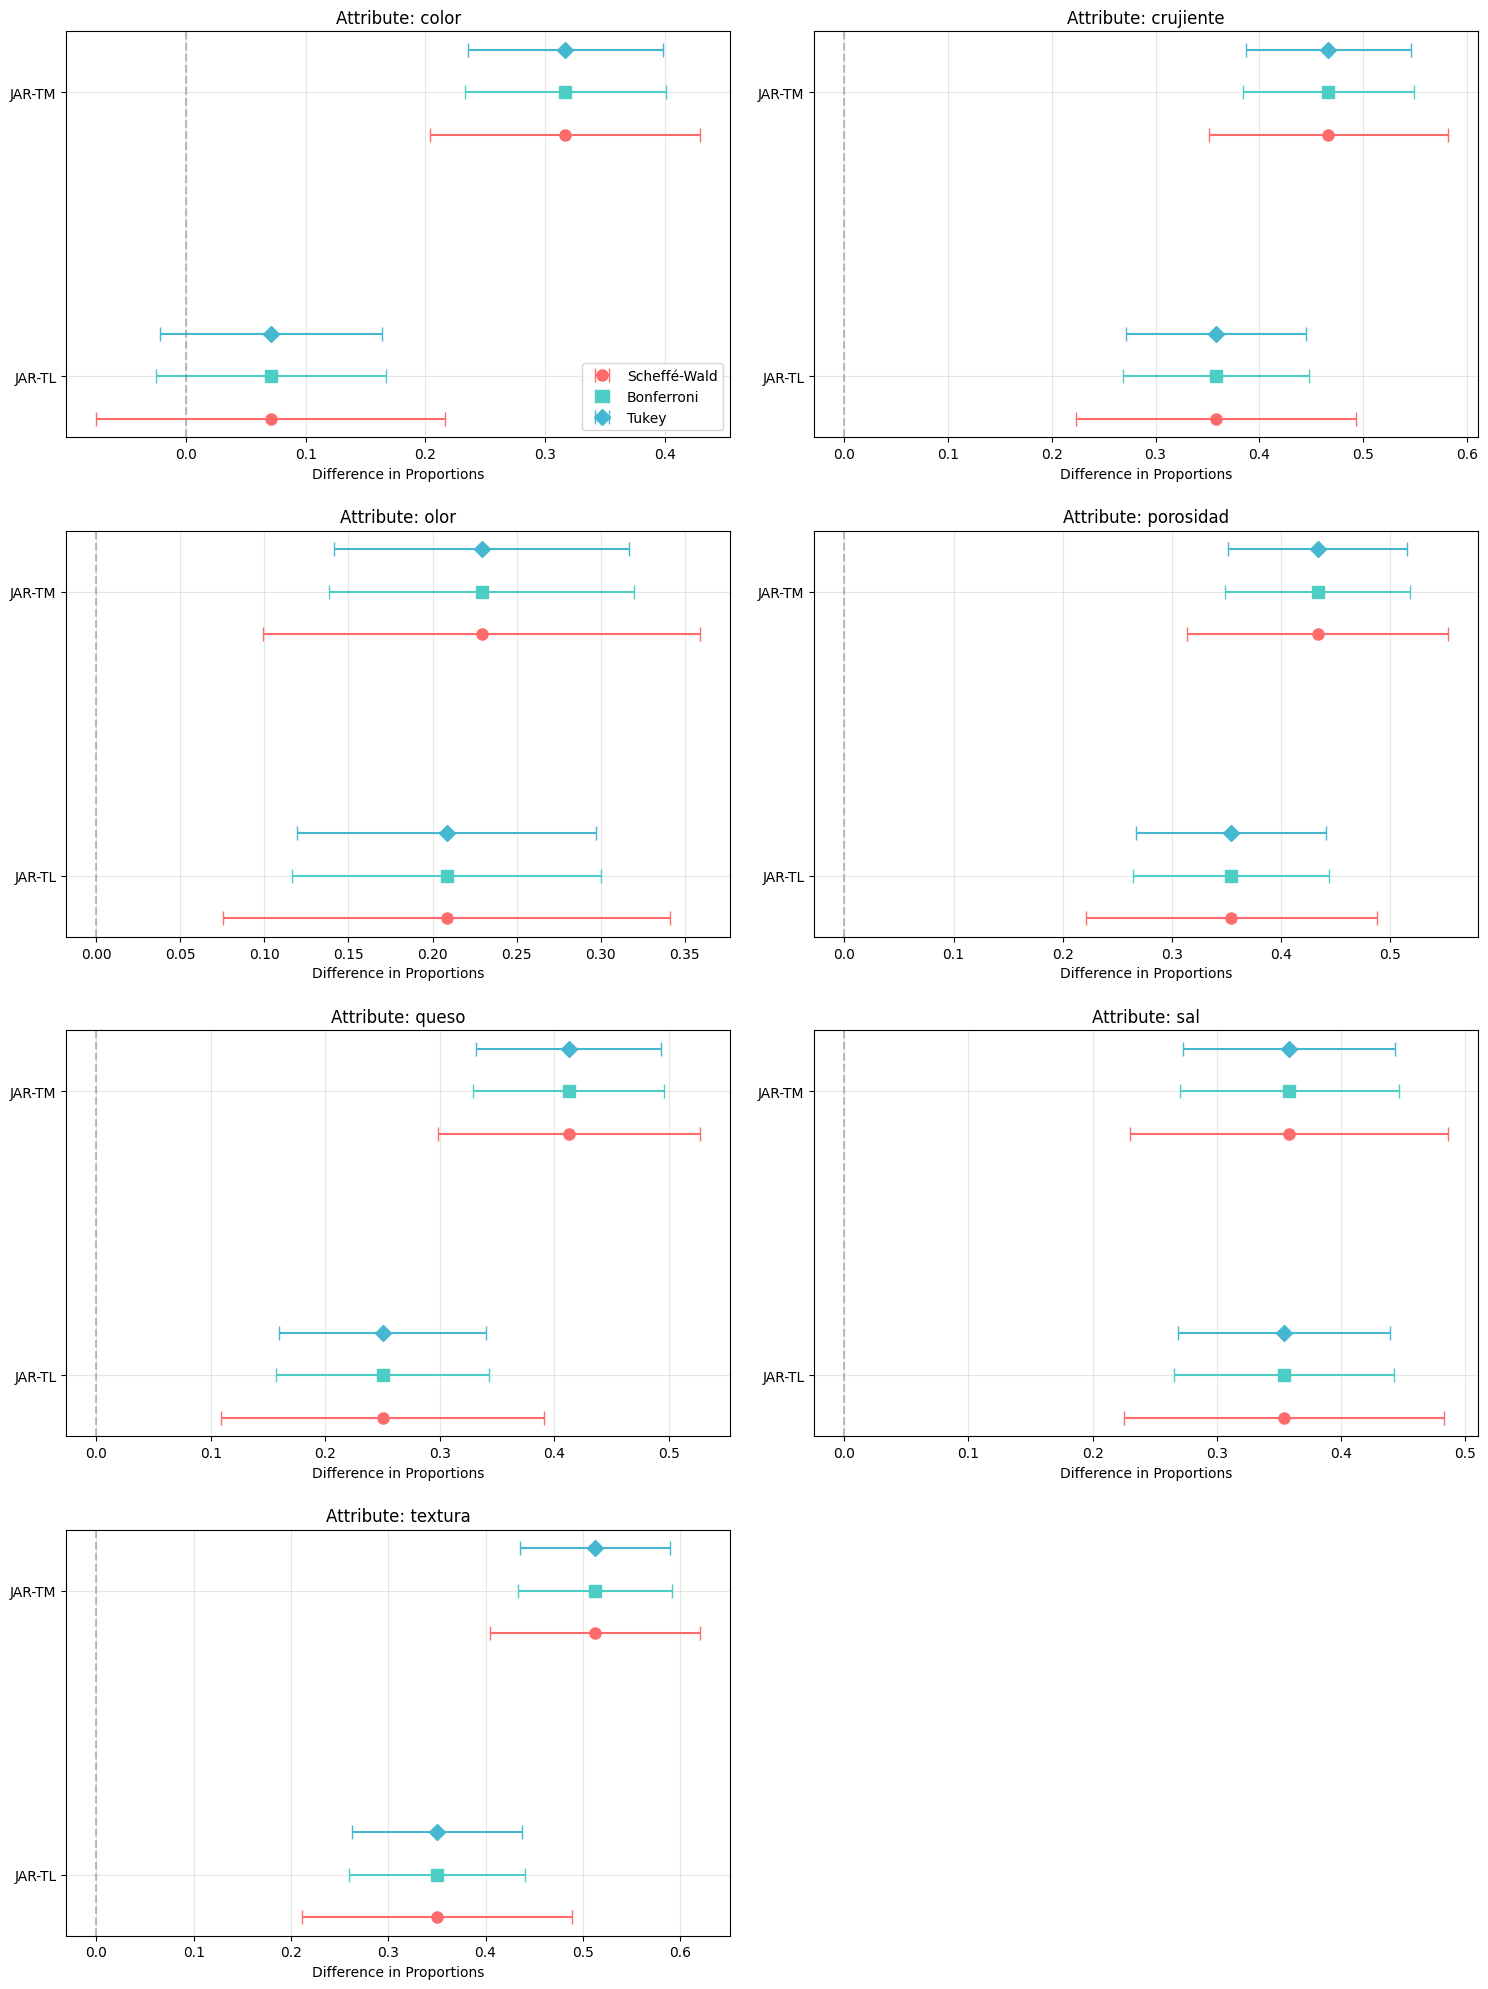
\includegraphics{implementation_files/implementation_12_1.png}
\caption{png}
\end{figure}

\begin{lstlisting}[language=Python]
import subprocess

subprocess.run('jupyter nbconvert --to markdown implementation.ipynb', 
                   shell=True, 
                   stdout=subprocess.DEVNULL, 
                   stderr=subprocess.DEVNULL, 
                   check=True)

subprocess.run('pandoc --listings -f markdown -t latex implementation.md -o implementation.tex', 
                   shell=True, 
                   stdout=subprocess.DEVNULL, 
                   stderr=subprocess.DEVNULL, 
                   check=True)
\end{lstlisting}

\begin{lstlisting}
CompletedProcess(args='pandoc --listings -f markdown -t latex implementation.md -o implementation.tex', returncode=0)
\end{lstlisting}
